\documentclass{article}
\usepackage{enumitem}
\usepackage{array}
\usepackage{subcaption}
\usepackage{graphicx}
\usepackage{subcaption}

\usepackage{color}
\usepackage[top=1in,bottom=1in,left=1.2in,right=1.2in]{geometry}
\usepackage{hyperref}
\usepackage[small]{titlesec}
\usepackage{booktabs}
\usepackage{colm2024_conference}
\usepackage{graphicx}
\usepackage[dvipsnames]{xcolor}
\usepackage{rotating}
\usepackage{pdflscape}
\usepackage{amsmath}

\newcommand{\todo}[1]{\textcolor{red}{\textbf{TODO:} #1}}

% Commenting
\newcommand{\eat}[1]{\ignorespaces}
%% Comment this line and uncomment the next to hide all comments
\newcommand{\xxcomment}[4]{\textcolor{#1}{[$^{\textsc{#2}}_{\textsc{#3}}$ #4]}}
\newcommand{\ta}[1]{\xxcomment{blue}{T}{A}{#1}}



\title{CS5787: Exercises 2 \\ \begin{small}\url{https://github.com/mitkrieg/dl-assignment-2}\end{small}}
\author{Mitchell Krieger \\ mak483@cornell.edu}

\date{}

\colmfinalcopy
\begin{document}
\maketitle

\section{Theory: Question 1 [10 pts]}

\begin{enumerate}[label=\alph*)]
    \item One way to deal with variable length input sequences is to pad sequences using a special token to be the same length as the length of the longest sequence. This method is simple and easy to implement approach makes it so that you can run inputs through transformations in the network, without loss of data. However, there is wasted computation and on the pads and if the inputs have a high variation in length it could negatively impact performance.
    \item To handle outputs of varying length we can append to the end of each input sequence a end of sequence (EOS) token. That way the model will be trained to predict when the next token should be the end of the sequence, thus indicating that the sequence should end. This could add to the total overall loss because if the model predicts EOS to0 soon or too late, that additional mistake contributes to the overal loss. 
\end{enumerate}

\section{Theory: Question 2 [10 pts]}

One major advantage of GRUs is that they are simplier than LSTMs because they have fewer gates and thus fewer parameters. This can make GRUs more efficent and faster to trian than LSTMs. Another advantage is that because there are fewer parameters, GRUs tend not to overfit as much as LSTMs do. 

\section{Theory: Question 3 [10 pts]}

In a LSTM cell there are 4 different gates each with its own learnable parameters. For a LSTM with an input of 200 and a hidden state of 200 each gate will have an input weight matrix of 200x200 so that the output of the gate will be a vector of 200 units. The same is true for the hidden state weight matrix. Lastly, each gate has a bias vector of 200. So for one gate there will be 200x200 + 200x200 + 200 = 80200 parameters. Since there are 4 gates, we can multiply this number by 4 to get the total number of 80200 x 4 = 320800 parameters in the LSTM cell.

\section{Theory: Question 4 [20 pts]}

\begin{enumerate}[label=\alph*.]
    \item
    \begin{equation*}
        \begin{aligned}
            \frac{\partial \epsilon_2}{\partial W_{xz}} &= \frac{\partial \epsilon_2}{\partial h_2} \frac{\partial h_2}{\partial z_2} \frac{\partial z_2}{\partial W_{xz}} \\
            &= \frac{\partial \epsilon_2}{\partial h_2} (h_1 - g_2) (z_2(1-z_2)) x_2
        \end{aligned}
    \end{equation*}

    \item
    \begin{equation*}
        \begin{aligned}
            \frac{\partial \epsilon_2}{\partial W_{hz}} &= \frac{\partial \epsilon_2}{\partial h_2} \frac{\partial h_2}{\partial z_2} \frac{\partial z_2}{\partial W_{hz}} \\
            &= \frac{\partial \epsilon_2}{\partial h_2} (h_1 - g_2) (z_2(1-z_2)) h_1
        \end{aligned}
    \end{equation*}

    \item
    \begin{equation*}
        \begin{aligned}
            \frac{\partial \epsilon_2}{\partial W_{xg}} &= \frac{\partial \epsilon_2}{\partial h_2} \frac{\partial h_2}{\partial g_2} \frac{\partial g_2}{\partial W_{xg}} \\
            &= \frac{\partial \epsilon_2}{\partial h_2} (1-z_2)(1-(g_2)^2) x_2
        \end{aligned}
    \end{equation*}

    \item
    \begin{equation*}
        \begin{aligned}
            \frac{\partial \epsilon_2}{\partial W_{hg}} &= \frac{\partial \epsilon_2}{\partial h_2} \frac{\partial h_2}{\partial g_2} \frac{\partial g_2}{\partial W_{hg}} \\
            &= \frac{\partial \epsilon_2}{\partial h_2} (1-z_2)(1-(g_2)^2)(r_2 \otimes h_1)
        \end{aligned}
    \end{equation*}

    \item
    \begin{equation*}
        \begin{aligned}
            \frac{\partial \epsilon_2}{\partial W_{xr}} &= \frac{\partial \epsilon_2}{\partial h_2} \frac{\partial h_2}{\partial g_2} \frac{\partial g_2}{\partial r_2} \frac{\partial r_2}{\partial W_{xr}} \\
            &= \frac{\partial \epsilon_2}{\partial h_2} (1-z_2)((W_{hg})^T \cdot h_1)(1-(g_2)^2)(r_2(1-r_2))(x_2)
        \end{aligned}
    \end{equation*}

    \item
    \begin{equation*}
        \begin{aligned}
            \frac{\partial \epsilon_2}{\partial W_{hr}} &= \frac{\partial \epsilon_2}{\partial h_2} \frac{\partial h_2}{\partial g_2} \frac{\partial g_2}{\partial r_2} \frac{\partial r_2}{\partial W_{hr}} \\
            &= \frac{\partial \epsilon_2}{\partial h_2} (1-z_2)((W_{hg})^T \cdot h_1)(1-(g_2)^2)(r_2(1-r_2))(h_1)
        \end{aligned}
    \end{equation*}
    
\end{enumerate}

\section{Practical [50 pts]}

In this experiment, our goal was to explore language modeling using the Penn Treebank Dataset with LSTMs and GRUs. The architecture used in this exploration was based on the “small” architecture from Zaremba et al.’s (2015) paper, Recurrent Neural Network Regularization. This architecture splits the data into 20 batches, sequentially traversing the dataset with a given sequence length (we used 20). The data is fed into a vocabulary embedding layer of size 200, followed by 2 layers of either LSTMs or GRUs, each with 200 hidden units. Finally, a fully connected layer of size 200 × vocab size outputs the logits.

We used stochastic gradient descent to optimize the cross-entropy loss of the model, along with a learning rate scheduler that, after a specified epoch number t, decreases the learning rate by a factor of n every subsequent epoch. For hyperparameter tuning of the initial learning rate, the epoch to start the decay, and the rate of decay, we used a manual trial-and-error approach until we found a set of hyperparameters that performed well on the validation set’s perplexity. We tracked our results using Weights and Biases.

In total, we built four models: two LSTM models and two GRU models, using the above architecture. For each RNN type, one model was implemented with dropout and the other with no regularization. In the models with dropout, we added dropout layers between the embedding and RNN layers, within the RNN layers, and between the RNN layers and the final fully connected layer. Dropout rates were set separately for the dropout within the RNNs and between layers. The same manual hyperparameter tuning process was used to adjust the dropout rates. A summary of the models, their best-performing hyperparameters, and their loss and perplexity metrics is presented below.


\begin{table}[ht]
    \centering
    \makebox[\textwidth]{
    \resizebox{1.4\textwidth}{!} {%
    \renewcommand{\arraystretch}{1.5}
    \begin{tabular}{|l|c|c|c|c|c|c|c|c|c|c|c|c|}
    \hline
    \rule{0pt}{15pt}
    RNN Type               & Epochs Trained & Starting \newline Learning Rate & LR Decay Rate & Start Decay at Epoch & Layer Dropout & RNN Dropout & Train Loss & Train Perplexity & Val Loss & Val Perplexity & Test Loss & Test Perplexity \\
    \hline
    LSTM no Regularization & 14             & 4                      & 0.5           & 10                   & -             & -           & 4.115      & 61.226           & 4.838    & 126.269        & 4.806     & 122.204         \\
    \hline
    LSTM with Dropout      & 25             & 6                      & 0.75          & 11                   & 0.5           & 0.2         & 4.111      & 61.030           & 4.597    & 99.171        & 4.562     & 95.794          \\
    \hline
    GRU no Regularization  & 14             & 1                      & 0.5           & 6                    & -             & -           & 4.330      & 75.963           & 4.804    & 122.055        & 4.777     & 118.583         \\
    \hline
    GRU with Dropout       & 25             & 1                     & 0.75          & 20                   & 0.5           & 0.2         & 4.202      & 66.688           & 4.687    & 107.651        & 4.650     & 104.543   \\
    \hline     
    \end{tabular} %
    }
    }
    
\end{table}

Looking at the performance metrics we see that on both models that were not regularized with drop out, the generalization error is worse: there's a delta between the train perplexity and the validation perplexity of ~65 the LSTM. Where as in the regularized LSTM, the generalization error is only around ~38 on the LSTM. This same behavior is not immediately apparent in the GRU, those models have a delta of 42 to 46. However, when you look at the convergence graphs below and also note that the GRU with dropout does have a better validation and test perplexity, we can begin to understand that dropout helped the GRU learn the dataset better.



\begin{figure}[ht] % Creates a floating figure
    \centering

    \caption{Convergence Graphs of Models}
    \label{fig:Convergence}

    % first row
    \begin{subfigure}[b]{0.45\textwidth}
        \centering
        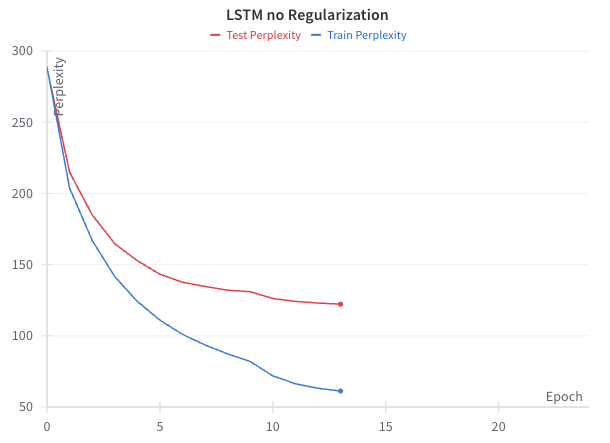
\includegraphics[width=\linewidth]{../src/lstm_noreg.png}
    \end{subfigure}
    \hfill
    \begin{subfigure}[b]{0.45\textwidth}
        \centering
        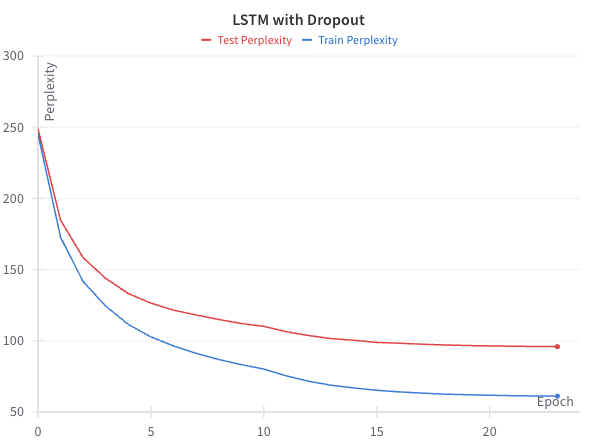
\includegraphics[width=\linewidth]{../src/lstm_drop.png}
    \end{subfigure}
    
    % second row
    \vskip\baselineskip
    \begin{subfigure}[b]{0.45\textwidth}
        \centering
        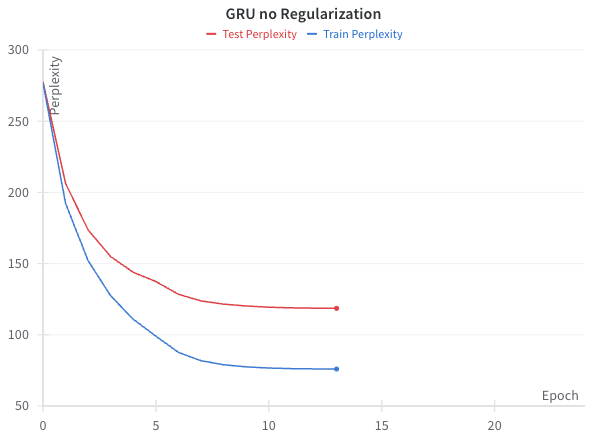
\includegraphics[width=\linewidth]{../src/gru_noreg.png}
    \end{subfigure}
    \hfill
    \begin{subfigure}[b]{0.45\textwidth}
        \centering
        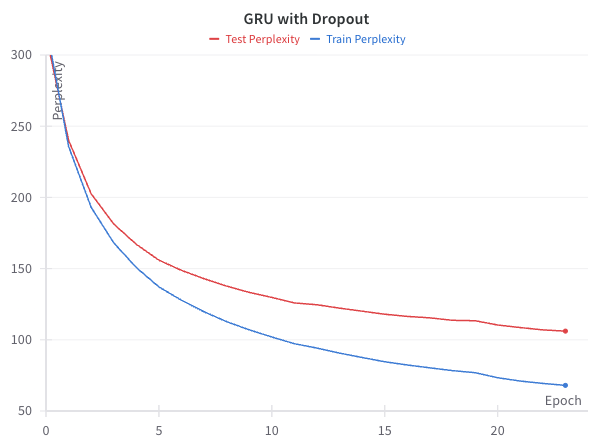
\includegraphics[width=\linewidth]{../src/gru_drop.png}
    \end{subfigure}
\end{figure}

Consider how quickly the gap between train and test perplexity on the GRU without regularization became within a few epochs and then rapidly began to plateau. This is a sign that the model may have been overfitting to the train set and would perhaps only have gotten worse if it had not been stopped at the 13th epoch. Where as in the GRU with dropout, the train and test perplexities are much closer together at the 13th epoch. In addition, while it was stopped at the 25th epoch, it hasn't quite yet completely plateaued and probably could have gained a bit more performance if let run for a bit longer. 

We can observe a similar behavior in the LSTM convergence graphs although the LSTM without regularization gets wider even faster than the GRU does. This is perhaps because there are many more learnable parameters in an LSTM than there is in a GRU because an LSTM has an additional gate. Because of this it is particularly important when using LSTMs and GRUs to regularize them to make sure that generalization error is minimized and the model performs well on the validation and tests sets, not just the training data.

When testing the model, it is also easy to see that although we've been able to bring down the perplexity score a decent amount the output of the model doesn't present as true natural language. This makes sense for such a simple architecture. A better language model would probably require additional RNN layers and/or more advanced architectures like encode-decoder networks with attention or transformers.

\end{document}